\documentclass{article}
\usepackage[utf8]{inputenc}


\title{Causal mediation in the presence of measurement error and baseline exclusion}
\author{Sicheng Hao}
\date{April 2021}

\usepackage{natbib}
\usepackage{graphicx}
\usepackage{color}
\usepackage{graphicx}
\usepackage{tikz}

\begin{document}

\maketitle

\section{Introduction}


Randomized Controlled Trials (RCTs) are considered as the gold standard for estimating the unbiased causal effect. However, the unbiased estimation doesn’t  bring insightful information about the causal mechanisms, which the goal of the investigation switched from how to why. Causal mediation analysis based on mediation analysis framework, gained popularity gradually among Epidemiological and biomedical researchers in the last 20 years. However, when applying causal mediation in complex biological systems such as the human body, the challenge of obtaining unbiased estimation still reminds. 

A typical RCT dataset contains randomly assigned treatment, biomarkers measurement at the baseline level and follow-up, and the target outcome.  The treatment effect can be obtained by comparing the outcome between the treatment and control groups. In causal mediation analysis, the treatment effect, also known as total effect (TE), is divided into two parts. One path through the target mediator is called Natural Indirect Effect (NIE). And the one working directly from treatment to outcome is called Natural Direct Effect (NDE). \cite{vanderweele2015explanation} The fundamental objective of causal mediation analysis in RCT is to compare the levels of post-randomization biomarker between patients in the treatment group and control group. 

The problem of using biomarkers as mediators is their time-varying nature. Many biomarkers, such as proteins and lipids, are measured in a single time shot. In fact, the effect of the biomarker is often associated with the cumulation of continuous value. For example, a patient with high-density cholesterol averaging 50mg/dl could have measurements ranging from 30mg/dl to 70mg/dl. \cite{barnett2005regression} In epidemiology, such phenomenons are called measurement errors. \cite{carroll2006measurement} The term doesn’t necessarily indicate an error in the measurement process but generally means the measured biomarker fluctuates randomly around the underlying mean. Fortunately, the measurement error problem is a well-researched model. Le cassis et al. proposed several scenario of where measurement error could happen in causal mediation analysis and proposed solution. \cite{le2012quantification}

However, in some clinical trials, specific biomarkers are excluded at the baseline. Such a selection combined with measurement error creates a new potential source of bias in addition to the bias caused by measurement error. This combination will also cause a phenomenon called regression towards the mean (RTM), a well-studied area. However, the existing biomarker RTM adjusting method often focused on the effect from treatment to the biomarker. No relevant work has been found to correct bias in causal mediation analysis caused by measurement error and selection at baseline in an RCT. 



\section{Background}

\subsection{Regression toward the mean}

The regression toward the mean (RTM) effect has a long history that could trace back to more than one hundred years ago identified by Francis Galton. The phenomenon can be summarized as in a variable with random variation, condition on extreme measurement, the following measures will present a trend toward the center of the distribution. The identification of RTM in an RCT is as simple as performing a t-test between the follow-up measures side-by-side with the baseline measures in the control group. The Follow-up group will have mean measurements closer to the population mean before selection and often increased variance. 

Notice the RTM effect has two components, random variation, and selection. Random variation and measurement error are interchangeable at a certain level. In the following text, random variation is used to describe the characteristics of a random variable to another; measurement error is used to describe aspects of a biomarker in which the average or cumulative value affects the target outcome, but such value cannot be directly measured.

\subsection{Classical measurement error in regression model}

In the classical measurement error framework, we assume X is the actual value, U is the random error centered at 0, and W is the observed measurement. Z is all the other covariates in vector form. 

\begin{figure}[h]
\centering
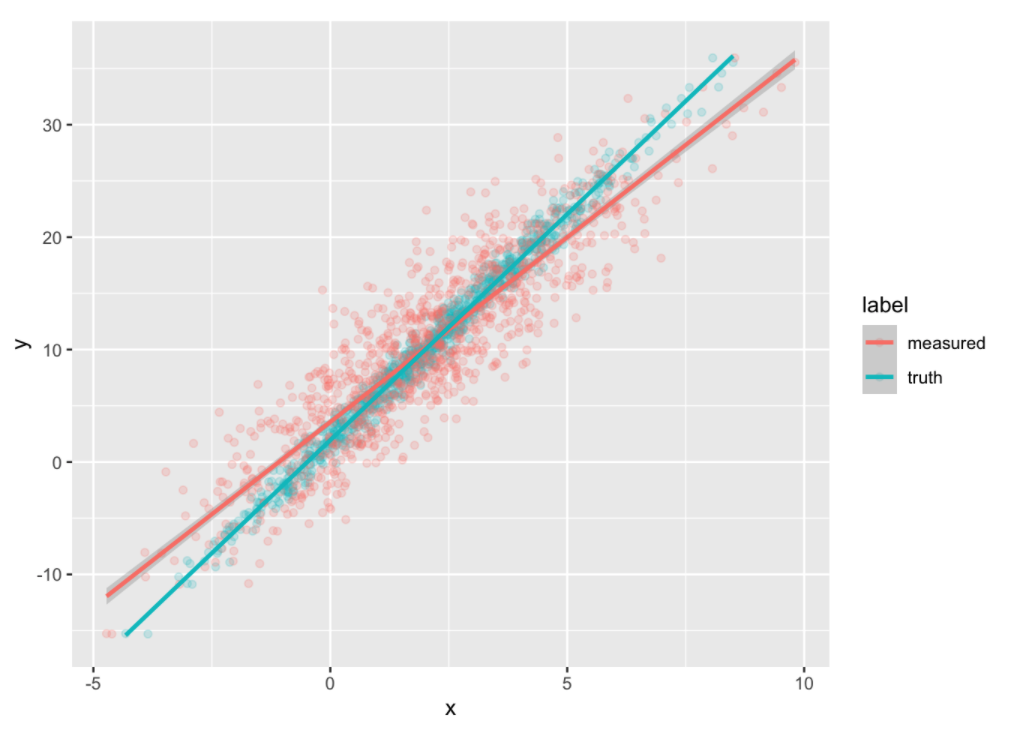
\includegraphics[width = 10cm,height = 8cm]{figure-1.png}
\caption{Example of measurement error on x causing regression coefficient to be biased}
\label{fig1}
\end{figure}


%1
\begin{equation}
W = X + U, U \sim Normal(0, \sigma_u)
\end{equation}

In this scenario, the objective of regression can be written as

%2
\begin{equation}
Y = \beta_0 + \beta_x  X + \beta_{z}^t Z + \epsilon
\end{equation}

Coefficients $\beta_x$ can be estimated using regression function

%3
\begin{equation}
Y = \beta_0^* + \beta_{w}  W + \beta_{z}^{t*} Z + \epsilon
\end{equation}

Let 

%4
\begin{equation}
\lambda = \frac{\sigma_{x|z}^2}{\sigma_{x|z}^2 + \sigma_{u}^2}
\end{equation}


%5
\begin{equation}
\beta_x = \beta_{w} \lambda
\end{equation}



Where $\lambda$ is the variation in W explained by X. Note when X is independent from Z:
 
%6
\begin{equation}
\lambda = \frac{\sigma_{x}^2}{\sigma_{x}^2 + \sigma_{u}^2}
\end{equation}

%explain RCT x independent from z




\subsection{Classical measurement error in survival analysis}

In causal mediation analysis with time-to-event data.  \cite{vanderweele2011causal} Given a general form of accelerated failure time time  (AFT) model

%7
\begin{equation}
log(T) = \beta_0 + \beta_x   X + \beta_{z}^t Z + \epsilon
\end{equation}


Parameter can be estimated in the same procedure as in section 2.2.



\subsection{Measurement error with truncation}

\begin{figure}[h]
\centering
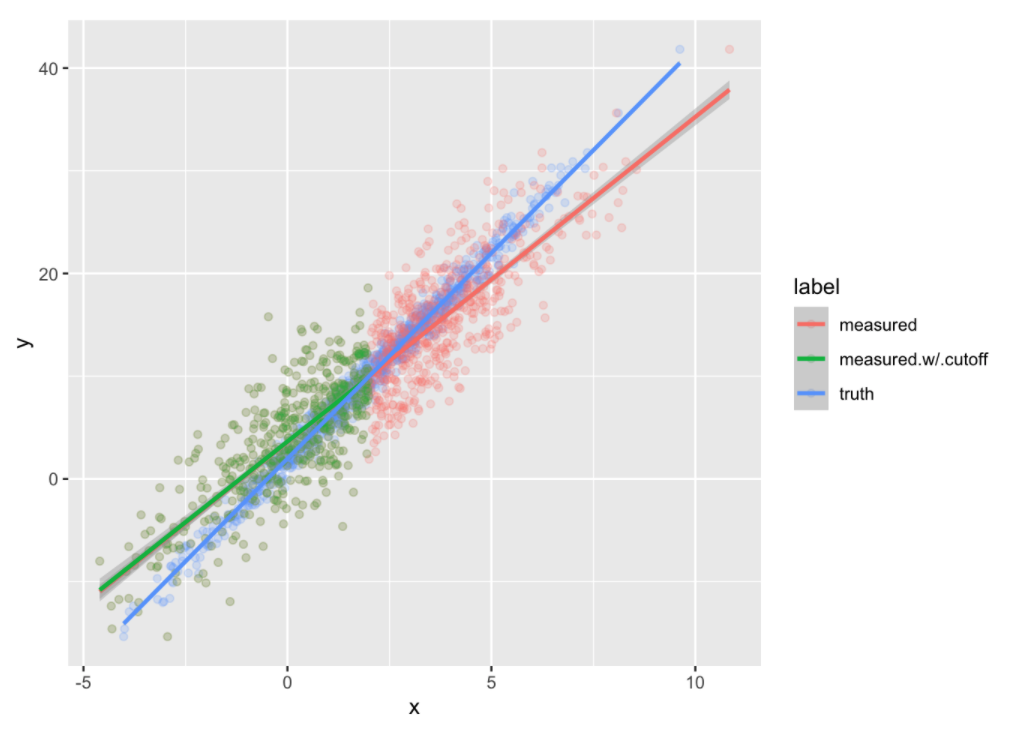
\includegraphics[width = 8cm,height = 6cm]{figure-2.png}
\caption{Example of measurement error with truncation on the measurement}
\label{fig2}
\end{figure}



\begin{figure}[h]
\centering
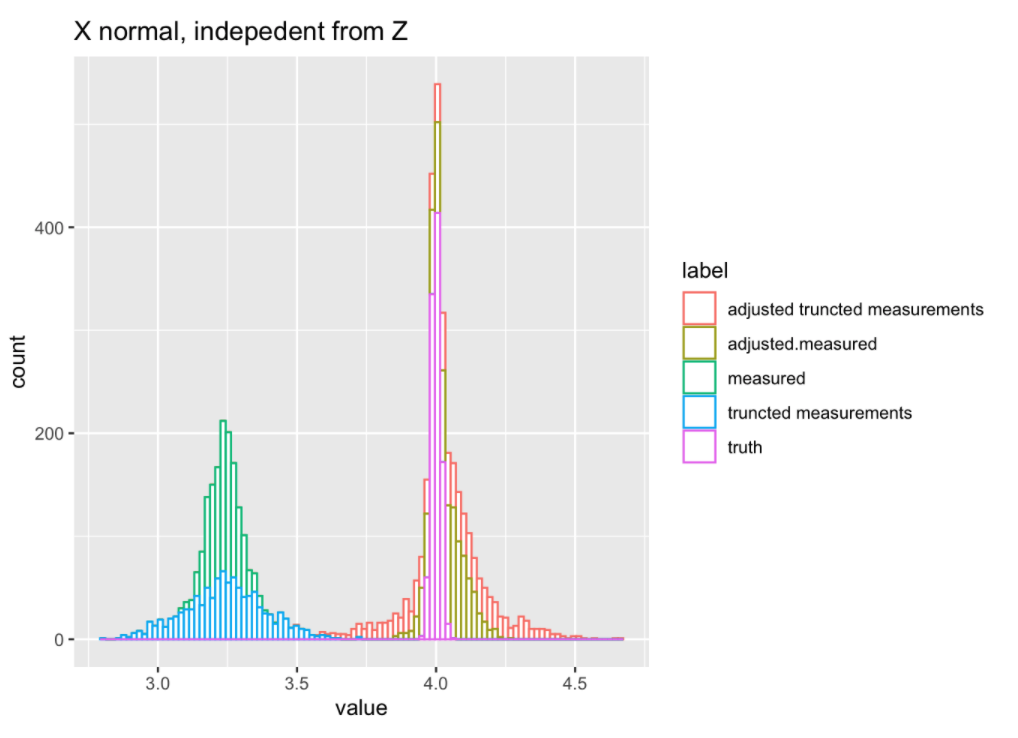
\includegraphics[width = 8cm,height = 6cm]{figure-3.png}
\caption{1000 simulated parameter estimation for X in different cases, X is normally distributed. }
\label{fig3}
\end{figure}

Figure-2 shows a simulated situation where the measurement W is truncated with only values below average. In Figure-3, we can see the bias on the regression coefficient due to measurement error, and truncation on measurement can be adjusted. However, the adjustment method of truncation only creates unbiased results when X is normally distributed. 


\pagebreak
\clearpage

\section{Method}

\subsection{Causal Mediation Analysis}

Causal mediation analysis quantifies the extent to which the total effect of an intervention (TE) splits into the effect produced by a known mediator, also called natural indirect effect(NIE), and the effect produced by other means, also known as the natural direct effect(NDE). NDE is the difference between TE and NIE indicates the presence of additional (and potentially novel) mechanisms that connect the intervention to the outcome.\newline

Causal mediation analysis required sequential ignorability, in parametric models, the assumption could translate to:\newline

Assumption 1:  No hidden exposure-outcome confounding\newline

Assumption 2:  No hidden mediator-outcome confounding\newline

Assumption 3: No hidden exposure-mediator confounding\newline

Assumption 4: No mediator–outcome confounding that is affected by the exposure\newline

Let Y be the outcome variable, A be the treatment, M be the mediator and C be the list of covariates.\newline


%8
\begin{equation}
E (M|A = a,C = c) = \beta_0+\beta_1 a+ \beta_2^{'} c
\end{equation}


%9
\begin{equation}
E (Y |M = m,A = a,C = c) = \theta_0+\theta_1 a+ \theta_2 m + \theta_3 a m + \theta_4^{'} c
\end{equation}

And then the direct effect and indirect effect can be written as:

%10
\begin{equation}
NDE = (\theta_1 + \theta_3 \beta_0 + \theta_3 \beta_1 a^* + \theta_3 \beta_2^{'} c)(a - a^*)
\end{equation}

%11
\begin{equation}
NIE = (\theta_2 \beta_1 + \theta_3 \beta_1 a)(a - a*)
\end{equation}


Causal mediation analysis have no problem working with time-to-event outcome. With one additional assumption:\newline

Assumption 5:  Mediator happened before outcome.\newline

%Compare with proportion hazard (PH) model are biased with common outcome in mediation analysis due to non-collapsibility , accelerated failure time (AFT) model are able to handle both rare and common outcome.

When mediator is continuous and the outcomes are time-to-event, parametric model could be written as:\


%12
\begin{equation}
M =  \beta_0+\beta_1 a+ \beta_2^{'} c + \epsilon
\end{equation}



%13
\begin{equation}
log(T) = \theta_0+\theta_1 a+ \theta_2 m + \theta_3 a m + \theta_4^{'} c + v \epsilon
\end{equation}



%14
\begin{equation}
NDE = exp((\theta_1 + \theta_3 (\beta_0 + \beta_1 a^* +  \theta_2^{'} c + \theta_2 \sigma^2))(a - a^*) + 0.5 \theta_3 ^2 \sigma^2 (a^2 - a^{*2}))
\end{equation}



%15
\begin{equation}
NIE = exp((\theta_2 \beta_1 + \theta_3 \beta_1 a)(a - a*))
\end{equation}


\subsection{Mediation with measurement error}

When exposure-mediator interaction term does not exist , measurement in the mediator can be addressed using the classical measurement error\cite{le2012quantification}.Let $\tilde M $ be the mediator value measured and M the the true value, and U be the error term with normal distribution centered around zero. Note the total effect and effect of exposure to mediator will not affected by the measurement error in the mediator. \cite{carroll2006measurement}\cite{le2012quantification}


\begin{figure}[h]
\centering
\begin{tikzpicture}[->,auto,node distance=3cm,
   thick,main node/.style={draw,font=\bfseries}]

\tikzstyle {edge} = [->, thick];

\node[text centered] (a) at (0,0){$A$};
\node[text centered] (m) at (3,0){$M$};
\node[text centered] (y) at (6,0){$Y$};
\node[text centered] (ms) at (3,-1){$M^*$};
\node[text centered] (u) at (3,-2){$U$};

%\draw [->] (t) -- (m);

\path (a) edge [bend left]  (y);
\path (a) edge []  (m);
\path (m) edge []  (ms);
\path (m) edge []  (y);
\path (u) edge []  (ms);

\end{tikzpicture}
\caption{DAG of mediation analysis with classical measurement error.  }
\label{dag1}
\end{figure}

Recall, real mediation M and measured mediation $\tilde M$ with measurement error U.\newline

%16
\begin{equation}
\tilde M = M + U, U \sim Normal(0, \sigma_u)
\end{equation}

Let $\lambda$ be the proportion of the total variance in $\tilde M $ explained by M. 


%17
\begin{equation}
\lambda = \frac{\sigma_{m|c}^2}{\sigma_{m|c}^2 + \sigma_{u}^2}
\end{equation}

%18
\begin{equation}
E(Y | A = a, \tilde M = \tilde m, C =c) = \theta_0+\theta_1 a+ \theta_2 \tilde m  + \theta_4^{'} c
\end{equation}


Rewrite (18) into into the form of AFT model: 
%19
\begin{equation}
log(T) = \tilde \theta_0+ \tilde \theta_1 a+ \tilde \theta_2 \tilde m + \tilde \theta_4^{'} c + v \epsilon
\end{equation}

The unbiased parameter $\theta_1$ and $\theta_2$ can be estimated using: 
%20
\begin{equation}
\theta_1 = \tilde \theta_1 - \tilde \theta_2(\frac{1}{\lambda}) \beta_1
\end{equation}

%21
\begin{equation}
\theta_2 = \frac{\tilde \theta_2}{\lambda}
\end{equation}



%22
%\begin{equation}
%NIE = exp((\theta_2 \beta_1 )(a - a^*))
%\end{equation}

%23
%\begin{equation}
%NDE = exp(\theta_1 (a - a^*))
%\end{equation}

\subsection{Mediation with measurement error and baseline exclusion }

\begin{figure}[h]
\centering
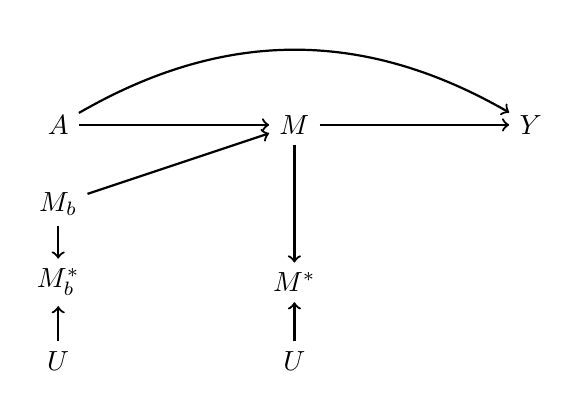
\begin{tikzpicture}[->,auto,node distance=3cm,
   thick,main node/.style={draw,font=\bfseries}]

\tikzstyle {edge} = [->, thick];

\node[text centered] (a) at (0,0){$A$};
\node[text centered] (m) at (3,0){$M$};
\node[text centered] (y) at (6,0){$Y$};
\node[text centered] (ms) at (3,-2){$M^*$};
\node[text centered] (m0) at (0,-1){$M_b$};
\node[text centered] (u) at (3,-3){$U$};
\node[text centered] (mbs) at (0,-2){$M_b^*$};
\node[text centered] (u2) at (0,-3){$U$};

%\draw [->] (t) -- (m);

\path (a) edge [bend left]  (y);
\path (a) edge []  (m);
\path (m) edge []  (ms);
\path (m) edge []  (y);
\path (u) edge []  (ms);
\path (m0) edge []  (mbs);
\path (m0) edge []  (m);
\path (u2) edge []  (mbs);

\end{tikzpicture} 
\caption{DAG of mediation analysis with classical measurement error and baseline exclusion.  }
\label{dag2}
\end{figure}


In the situation where measurement error existed in the mediator (Figure-5). When we force an exclusion either based on the measured mediator or variable that correlated with the mediator, additional bias could be introduced. The term "selection" or "exclusion" are referring to the data collection which separate from the data generating process and the term "truncation" are referring to the distribution of data. The two term are interchangeable in high-level. \

Recall (20) and (21), the adjustment of parameters used in causal mediation analysis depend on the parameter $\lambda$, which depend on $\sigma^2_{m|c}$ which will affected by baseline exclusion. 



\begin{figure}[h]
\centering
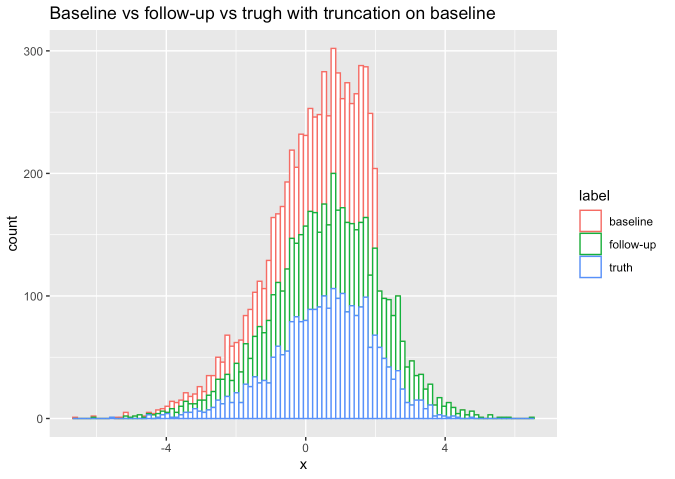
\includegraphics[width = 8cm,height = 6cm]{figure-4.png}
\caption{Simulated data: distribution of true data, baseline(truncated), follow-up }
\label{fig4}
\end{figure}



\subsection{New adjustment formula}

Recall (17), $\lambda$ is the variation of measured mediator explained by the true mediator. In a truncated situation, the true value is not likely to be as same as before. Assume $\mu_m $, $\sigma_{m|c}$ and $\sigma_u$ are known, a simulated approach could be used to estimate  $\sigma_{m_{new}|c}$ and the new $\lambda$ after truncation ($\lambda_{new}$)

%24
\begin{equation}
\lambda_{new} = \frac{\sigma_{m_{new}|c}^2}{\sigma_{m_{new}|c}^2 + \sigma_{u}^2}
\end{equation}


A simulation study is conducted to emulated data generate with RCT design where treatments are randomly assigned to two balanced group.  The true mediator post-randomization $M \sim Normal (\mu, \sigma_{m}) $ and it's measurement $\tilde M \sim Normal (M, \sigma_U)$, are affected by a selection on the baseline measurement of $\tilde M$. Figure-6 shows the distribution of the three variation above, we can see between baseline and follow-up measurements, RTM emerge since the mean of follow-up distribution shift right. 

Figure-7 and Figure-8 is the causal mediation parameter $\theta_1$ and $\theta_2$ under the original and new adjustment formula.


\begin{figure}[h]
\centering
\includegraphics[width = 8cm,height = 6cm]{figure-5.png}
\caption{1000 Simulation of theta1}
\label{fig5}
\end{figure}



\begin{figure}[h]
\centering
\includegraphics[width = 8cm,height = 6cm]{figure-6.png}
\caption{1000 Simulation of theta2 }
\label{fig6}
\end{figure}



\subsection{Covariates dependent with mediator}


In the previous formula, we know that when covariate c and m are not independent then


%21
\begin{equation}
\sigma^2_{m}  \ge \sigma^2_{m|c}
\end{equation}

%22
\begin{equation}
 \lambda = \frac{\sigma_{m|c}^2}{\sigma_{m|c}^2 + \sigma_{u}^2} \le \frac{\sigma_{m}^2}{\sigma_{m}^2 + \sigma_{u}^2} = \lambda^*
\end{equation}



Therefore, in cases that we are not able estimate $\sigma^2_{m|c} $ directly, we can still conclude an upper bound of the adjustment coefficient $\lambda$ using $\sigma^2_m$. Additionally, we can calculate the direction of reminding bias in  $\theta_2$. Since $\lambda \le \lambda^* \le 1$, then 


%23
\begin{equation}
|\theta_2| \ge   |\theta_2^*|  \ge |\tilde \theta_2|
\end{equation}



\subsection{Exposure-mediator interaction with categorical exposure}

Exposure-mediator interactions in the mediation model is important to obtain the unbiased result. However, estimation of coefficient of the interaction term $\theta_3$ using the method based on regression with interaction term is rather difficult, when measurement error exist. There hasn't been any previous literature mentioning the measurement error in mediation analysis with exposure-mediation interaction, as well as truncation on mediator on top of the interaction. 

A short cut approach can be taken using the fact that exposure is categorical, binary in most of the RCT. Data can be stratified into two groups and modeled differently.

Recall (), when exposure-mediator interaction term exist, and the exposure has two level 0 and 1, the regression model on Y can be written as:


%23
\begin{equation}
E (Y |M = m,A = a_0,C = c) = \theta_0+\tilde \theta_1 a+ \tilde \theta_2 m + \tilde \theta_4^{'} c
\end{equation}



%23
\begin{equation}
E (Y |M = m,A = a_1,C = c) = \tilde \theta_0+\tilde \theta_1 a+ (\tilde \theta_2 + \tilde \theta_3) m + \theta_4^{'} c
\end{equation}


Then we can use (21), to estimates

%23
\begin{equation}
 \lambda = \frac{\sigma_{m|c}^2}{\sigma_{m|c}^2 + \sigma_{u}^2}
\end{equation}



%23
\begin{equation}
\theta_3 = \frac{(\tilde \theta_2 + \tilde \theta_3)}{\lambda} - \theta_2
\end{equation}


Similar in 3.4 if covariates and mediator are not independent, $\theta_3$ have the similar direction of bias compare with $\theta_2$ which is biased towards the null. Given $\beta_1$ is unbiased, we can conclude the NIE in equation (25) is always going to biased towards the null. Further more using the fact NDE is the different between TE and NIE, we are able to correct the proportion of mediation with the proposed method. 

\subsection{Degrees of selection, a simulation study }

Simulations were designed to investigate the direction of the bias of the measurement error in mediator with truncation with the presents of exposure-mediator interaction and the degree of selection on the parameter. Exposure-mediator interaction terms are being considered extensively, where a factorial design is implemented with regard to data generated and the model used. 

Conclusion in(25) is being confirmed in the simulation (Figure-10), where when measurement error existed in the mediator, higher degree of selection on baseline will result a higher bias for $\theta_2$ and $\theta_3$ (Figure-11) as well as NIE to be biased towards the null.

Additional, in Figure-9 although $\theta_1$ is not being affected unless being modeled without the exposure-mediator interaction term. The NDEs will be affected since selection affected NIE and TE stays the same.

\begin{figure}[h]
\centering
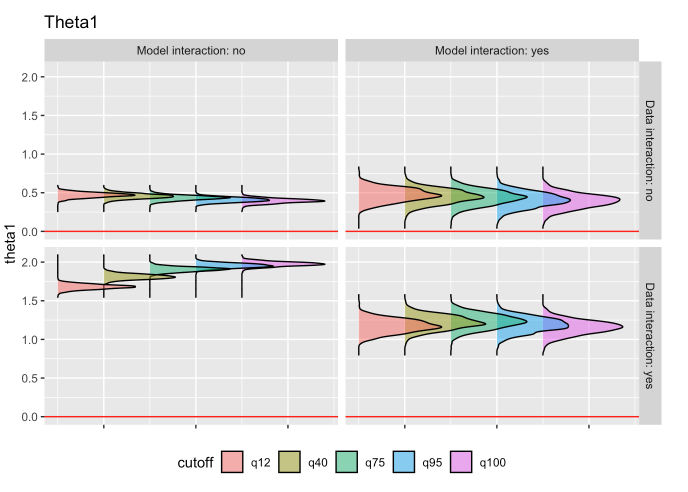
\includegraphics[width = 8cm,height = 6cm]{figure-7.png}
\caption{Theta1 under different interaction situation in the model and data with truncation}
\label{fig7}
\end{figure}

\begin{figure}[h]
\centering
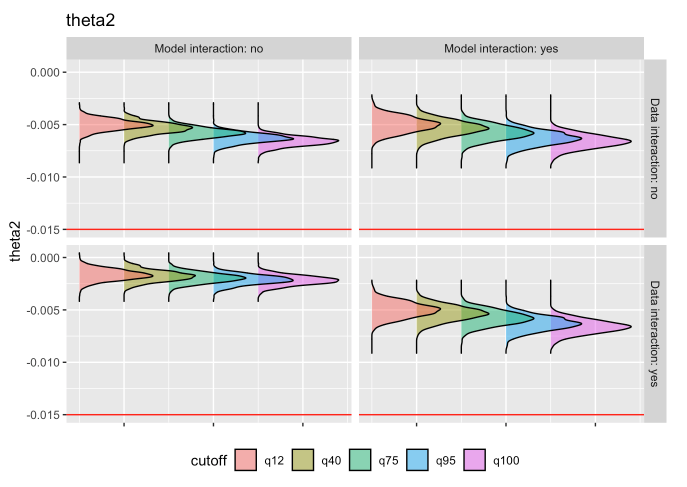
\includegraphics[width = 8cm,height = 6cm]{figure-8.png}
\caption{Theta2 under different interaction situation in the model and data with truncation} 
\label{fig8}
\end{figure}


\begin{figure}[h]
\centering
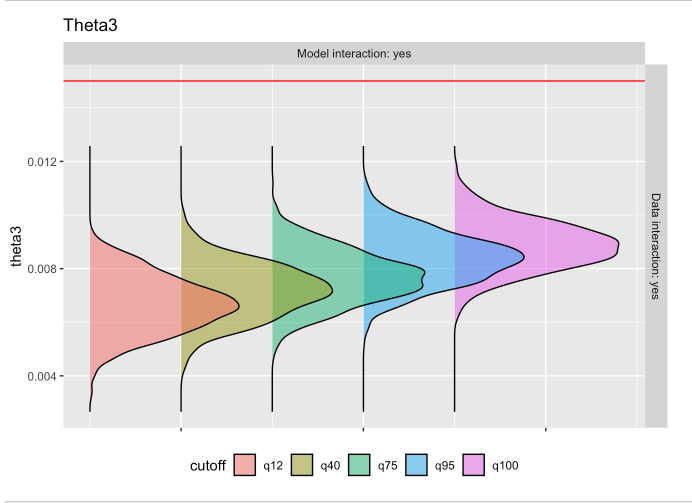
\includegraphics[width = 8cm,height = 6cm]{figure-9.png}
\caption{Theta3 when truncation present.}
\label{fig9}
\end{figure}




\pagebreak
\clearpage

\section{Application}

\subsection{Real world data}

In an RCT trial with a statin drug as exposure, researcher exclude people with Low density lipoprotein cholesterol (LDLC) more than 130 mg/dL.\cite{ridker2008rosuvastatin}  The trial showed a significant treatment of statin in reduce the cardiovascular disease and mortality. All the biomarkers are measured both at baseline and follow-up. A significant decrease in LDLC is also observed as a result of the trial and LDLC are often considered the major pathway of statin drug. \cite{chen2000direct}\cite{stancu2001statins} Lipids are often have noticeable variation between measurements.  Figure-12 and Figure-13 show the presents of truncation likely resulted a regression towards the mean effect. 


In Chapter 2 and 3, we showed measurement error and baseline selection will create bias for causal mediation analysis and proposed a new way to adjust the bias. However, in order to estimate $\lambda_{new}$ mentioned in (22), we need to estimate $\sigma^2_{m_{new}}$ and $\sigma^2_u$ from data


\begin{figure}[h]
\centering
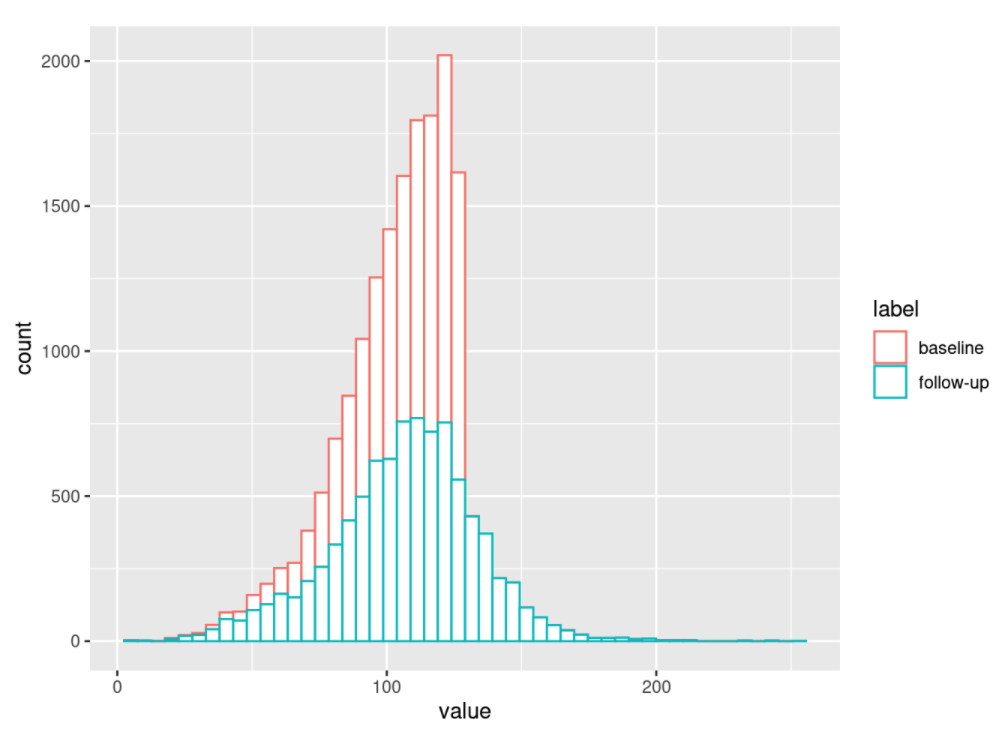
\includegraphics[width = 8cm,height = 6cm]{figure-10.png}
\caption{Histogram of LDLC measured in baseline and follow-up in the control group.}
\label{fig10}
\end{figure}

\begin{figure}[h]
\centering
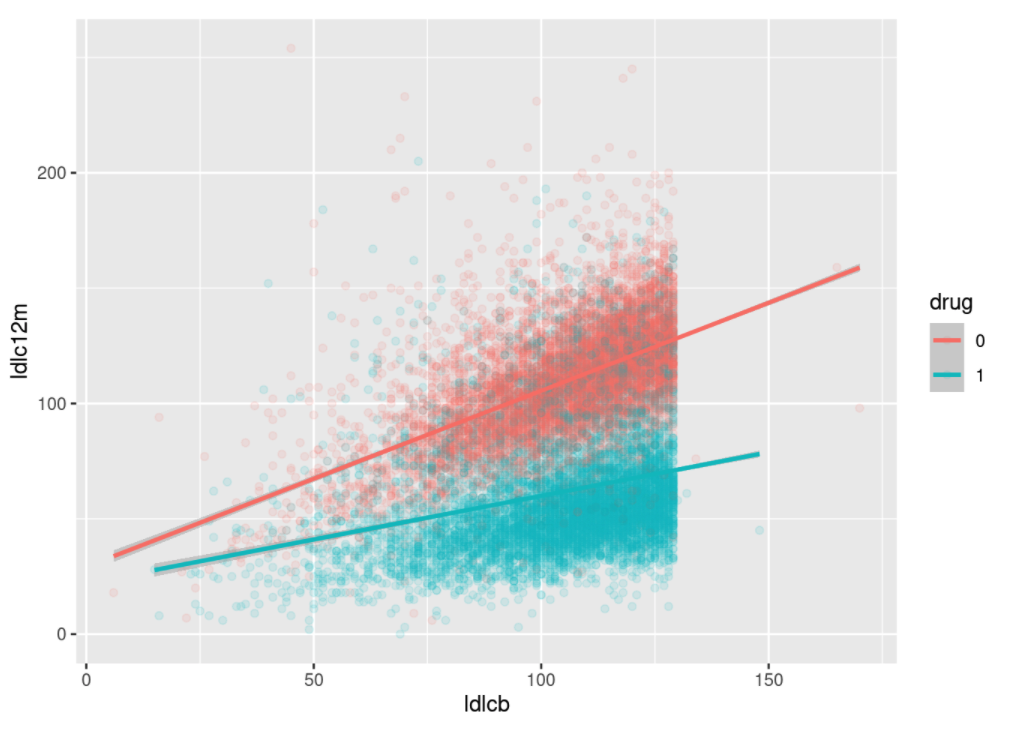
\includegraphics[width = 8cm,height = 6cm]{figure-11.png}
\caption{Point plot of LDLC measured in baseline and follow-up. Linear lines are fitted in each group. }
\label{fig11}
\end{figure}


\subsection{Estimation using the simulation}

A study using long term follow-up data showed the average of LDLC level in population has a mean around 116 and standard deviation of 14.2. \cite{takahashi2010lipid} Assume both average LDLC level and within person LDLC level measurement both follows normal distributions. We estimated the $\sigma_U$ around 16. After performing a simulation,  $\sigma^2_{m_{new}}$ is estimated to be 12.7 and $\lambda_{new}$ is around 0.38. 

\subsection{Results of causal mediation analysis}

When implementing causal mediation analysis on the trial data with LDLC at follow-up as the mediator, with a list of covariates that adjust such as, blood pressure, C-reactive protein, HDL, APOA, APOB, and smoking status. The odds ratio of NIE is 1.24, and odds ratio of NDE is 1.17, which results a proportion mediated of 0.623.

The NIE after adjustment is 1.77 and NDE after adjustment is 0.82, with proportion mediated of 1.39.  Although the NDE seems to have detrimental effect, the total effect is significantly positive. Due to several key parameters are not estimated using large dataset, above result needed to be carefully reviewed for clinical purpose. 


\begin{figure}[h]
\centering
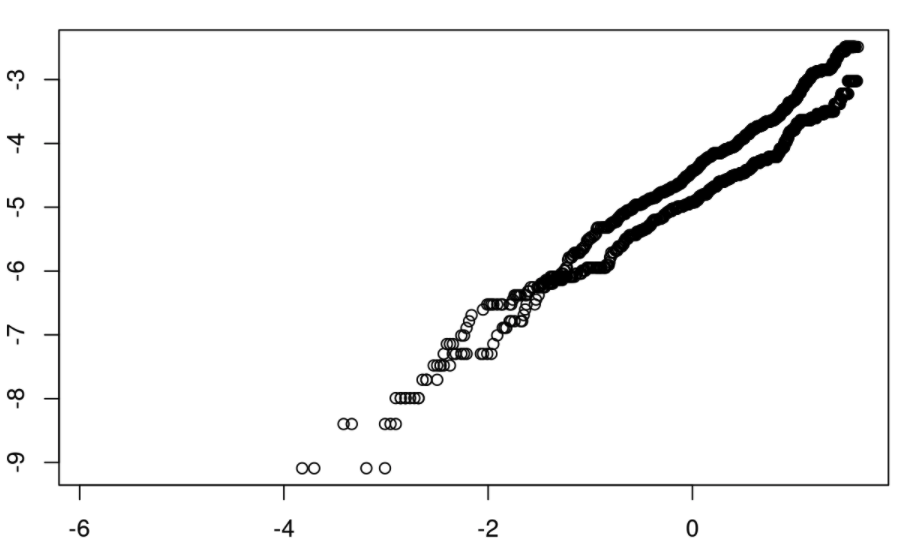
\includegraphics[width = 8cm,height = 6cm]{figure-12.png}
\caption{Assumption checking for survival analysis.  Log(-log(survival) vs. log(time). }
\label{fig12}
\end{figure}




\pagebreak
\clearpage


\section{Discussion}

\subsection{Key contibutions}

One of the most critical contributions of this research is that baseline exclusion or other truncation on the mediator would affect the results in addition to measurement error. And more extreme selection will further bias the results, where the original adjustment method wouldn’t obtain unbiased results. 

Another novelty coming from this research is the consideration of exposure-mediator interaction existed while adjusting for measurement error in mediators that previous research has no mention. Although the proposed solution didn’t address this problem fully from a theoretical perspective, only solved the cases when exposures are categorical, from an applicational viewpoint, most of the exposures in epidemiological and clinical studies are categorical. Furthermore, some estimates are difficult to acquire from real-world data due to the strong assumptions required for measurement error and adjustment and causal mediation analysis. The proposed solution can handle exposure-mediator interaction without demanding additional assumptions. 


\subsection{Weaknesses}

The most apparent weakness of the proposed adjustment solution is the estimation of $\sigma_U$ and  $\sigma_{m | c}$ and $\sigma_{m_{new}|c}$. Since such numbers cannot be estimated using data from the RCT alone. Additional study and metadata need to be acquired in order to estimate those parameters. Due to this reason, the result from chapter 4.3 is better served as a starting point of a new research project focused more on the clinical side of things in contrast to this thesis work which is inspired by a clinical problem but purely theoretical. 

From a methodological perspective, a flaw that the new adjustment didn’t address is when the mediator is normally distributed. Recall chapter 2, in order for the regression coefficient under truncation to work, the true distribution needs to be normal. This problem will also show up in the situations where baseline measurements are being truncated because an extreme truncation will deviate the true value from normal given it is before the truncation. 






\bibliographystyle{plain}
\bibliography{references}
\typeout{} 
\end{document}




